\documentclass[12pt, a4paper]{article}

\usepackage{fancyhdr}
\usepackage[left=4cm, right=4cm, top=4cm, bottom=4cm]{geometry}
\usepackage[utf8]{inputenc}
\usepackage[table]{xcolor}
\usepackage{hyperref}
\usepackage{amsmath}
\usepackage{enumitem}
\usepackage{graphicx}
\usepackage{booktabs}
\usepackage{subcaption}
\usepackage{xepersian}

\DeclareMathOperator*{\argmax}{argmax}
\DeclareMathOperator*{\argmin}{argmin}
\newcolumntype{L}{>{$}l<{$}} % math-mode version of "l" column type

\newcommand{\coursetitle}{یادگیری ماشین}
\newcommand{\doctitle}{تمرین چهارم}
\newcommand{\name}{محمدرضا غفرانی}
\newcommand{\studentno}{400131076}
\newcommand{\todaydate}{\today}

\settextfont{Sahel}
\setlatintextfont{Times Newer Roman}

\pagestyle{fancy}
\lhead{\textbf{\doctitle}}
\chead{\name}
\rhead{\todaydate}

\begin{document}

\begin{flushleft}
    \name \\
    \studentno \\
    \todaydate
\end{flushleft}

\begin{center}
    \huge
    \textbf{\coursetitle}
    \break
    \large
    \doctitle
\end{center}

% suppress the fancy header on the first page only
\thispagestyle{plain}

\section*{سوالات تشریحی}
\section*{سوال یک}

خوشه‌بندی انجام شده به همراه مراکز خوشه در شکل \ref{kmeans} آورده شده است.

\begin{figure}[h]
    \centering
    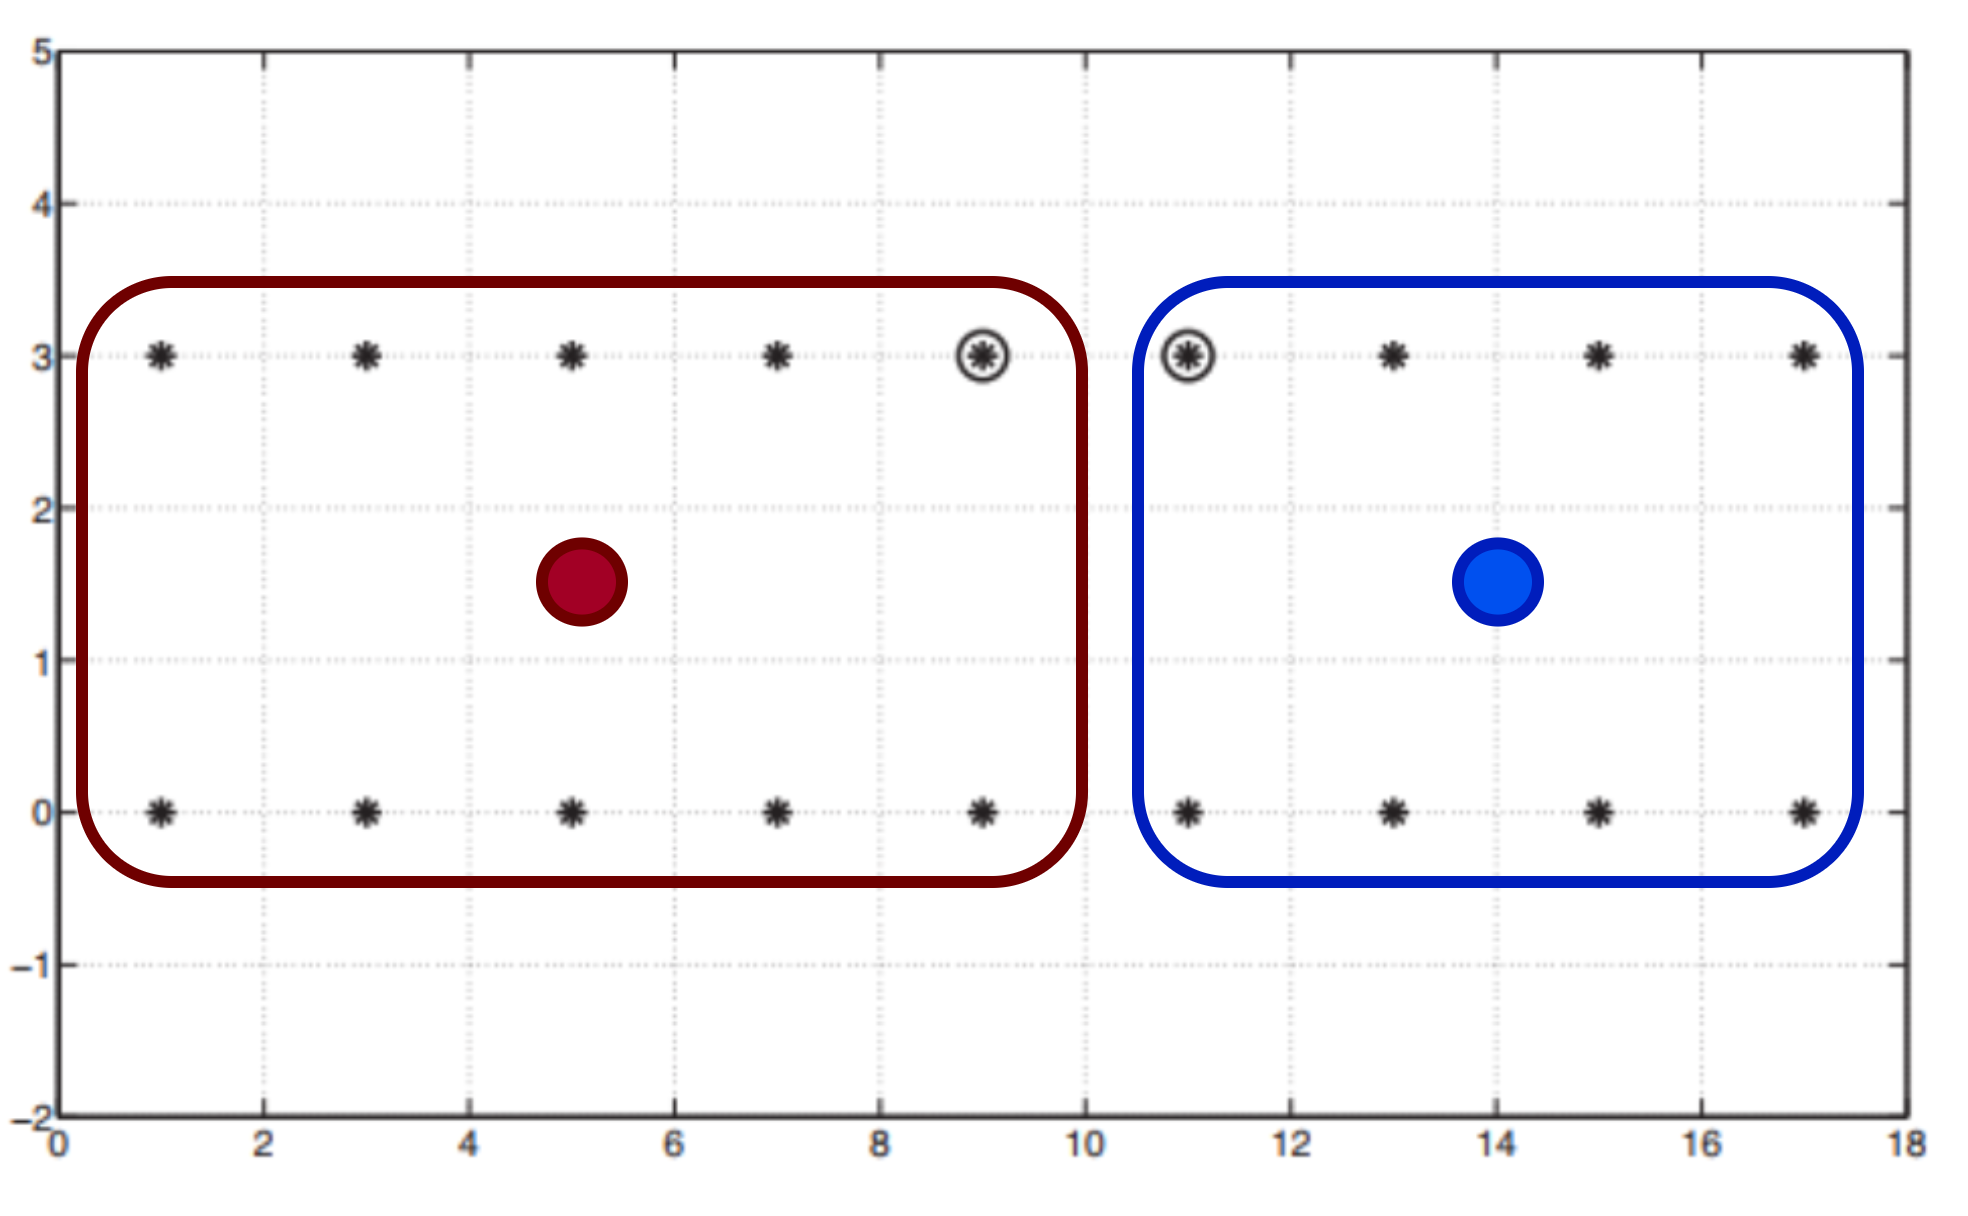
\includegraphics[width=0.8\linewidth]{images/long_answer/q1/kmeans.png}
    \caption{خوشه‌بندی انجام شده با \lr{kMeans}}
    \label{kmeans}
\end{figure}

\section*{سوال دو}

\begin{itemize}
    \item \lr{customer segmentation}: در این کاربرد مشتریان برحسب رفتاری که از خود نشان می‌دهند به چند
    دسته می‌شوند. همان‌طور که قابل پیش‌بینی است، مشتریان معمولا بدون برچسب هستند. بنابراین تنها راهکار تفکیک
    مشتریان با استفاده از الگوریتم‌های خوشه‌بندی است. در ادامه این خوشه‌بندی، معمولا چند داده از
    خوشه‌ها بررسی می‌شود تا برای خوشه برچسب مناسبی در نظر گرفته شده و سیاست‌های مناسبی برای هر دسته از کاربران در
    نظر گرفته شود.
    \item \lr{dimensionality reduction}: می‌توان از تکنیک زیر برای خوشه‌بندی داده‌ها استفاده کرد.
    با خوشه‌بندی داده‌ها را به $k$ دسته تقسیم کنیم. با فرض این که $k<d$، می‌توان فاصله هر داده تا این
    $k$ مرکز را محاسبه کرده و از این بردار حاصل شده برای نمایش داده‌ها استفاده کنیم. در این حالت داده‌ها از
    فضای $d$ بعدی به فضای $k$ بعدی منتقل می‌شوند.
    \item \lr{outlier detection}: برای شناسایی این داده‌ها می‌توان از خوشه‌بندی‌هایی نظیر \lr{DBSCAN} استفاده کرد
    که به پیوستگی بین داده‌ها بها می‌دهد. در این الگوریتم‌های خوشه‌بندی به صورت خودکار داده‌های نویز شناسایی شده
    و کنار گذاشته می‌شوند.
    \item \lr{image segmentation}: در این کاربرد نیاز است تا پیکسل‌های با رنگ یکسان شناسایی شوند. چرا که
    معمولا پیکسل‌هایی که رنگ آن‌ها با هم اختلاف اندکی دارد معمولا کنار یکدیگر بوده و متعلق به یک دسته هستند.
    با اجرای الگوریتم‌های خوشه‌بندی نظیر \lr{kMeans} این پیکسل‌ها به یک دسته نگاشت شده و \lr{segment}‌های
    تصویر شناسایی می‌شوند.
\end{itemize}

\section*{سوال سه}

برای انتخاب پارامتر \lr{MinPts} معمولا پیشنهاد می‌شود که بر اساس اندازه دادگان و دانش خبره تصمیم‌گیری شود.
هر چقدر اندازه دادگان پیش‌تر باشد، عدد بزرگتری برای \lr{MinPts} انتخاب می‌شود؛ به علاوه این که، فرد خبره
با توجه به درک بهتری که از روابط داده‌ها دارد عدد بهتری را می‌تواند برای \lr{MinPts} پیشنهاد دهد.

در ادامه برای پارامتر $\varepsilon$ پیشنهاد می‌شود که میانگین فاصله $k$ نزدیک‌ترین نقطه به هر نمونه
در نظر گرفته شود. برای پارامتر $k$ نیز همان مقدار پارامتر \lr{MinPts} استفاده می‌شود.

\section*{سوال چهار}

در الگوریتم \lr{Policy Iteration} یک سیاست و ارزش اولیه برای هر حالت در محیط در نظر گرفته می‌شود.
در گام‌های بعدی تلاش می‌شود با به‌روزرسانی ارزش‌های در نظر گرفته شده، سیاست‌ها به‌روز شود. این روند
تکرار می‌شود تا سیاست‌ها همگرا شود. در واقع تاکید این الگوریتم بر سیاست‌هاست و نه ارزش‌ها اما برای
به‌روزرسانی سیاست‌ها از ارزش‌ها را نیز به‌روز می‌کند.

در الگوریتم \lr{Value Itration} تاکید الگوریتم بر روی ارزش‌هاست و در هر مرحله تلاش می‌کند این ارزش‌ها را
به‌روز کند. هنگامی که ارزش‌ها به همگرایی می‌رسند، حال سیاست بهینه را از روی آن‌ها استخراج می‌کند.

\section*{سوال پنجم}

\subsection*{قسمت الف}

در ادامه توضیح مختصری درباره هر یک از این الگوریتم‌ها داده می‌شود.

\begin{itemize}
    \item \lr{Complete Linkage}: در این حالت برای ادغام دو دسته، فاصله بین دورترین نقاط آن‌ها در نظر گرفته می‌شود.
    به عبارت دیگر هر دو دسته‌ای که ماکزیمم فاصله بین نقاط دسته‌ها مینیمم باشد، با هم ادغام می‌شوند.
    \item \lr{Single Linkage}: در این الگوریتم برای ادغام دو خوشه، فاصله بین نزدیک‌ترین داده‌ها ملاک فاصله بین دو
    خوشه است. به عبارت دیگر هر دو دسته‌ای که مینیمم فاصله بین نقاط خوشه‌ها مینیمم باشد، با هم ادغام می‌شوند.
    \item \lr{Average Linkage}: در این روش خوشه‌بندی، میانگین فاصله بین نقاط دو خوشه ملاک فاصله بین دو خوشه است.
    به عبارت دیگر هر دو دسته‌ای که میانگین فاصله بین نقاط خوشه مینیمم باشد، با هم ادغام می‌شوند.
\end{itemize}

در ادامه تفاوت بین روش‌ها از نظر پیچیدگی زمانی و حساسیت به داده پرت بررسی می‌شود.
الگوریتم \lr{Average Linkage} نسبت به دو الگوریتم دیگر پیچیدگی بیشتری برای محاسبه فاصله داشته و بالطبع
از لحاظ محاسباتی پیچیده‌تر است. اما این الگوریتم به دلیل میانگین‌گیری حساسیت کمتری به نویز دارد. در بین دو الگوریتم
دیگر حساسیت الگوریتم \lr{Single Linkage} به نویز بیشتر از \lr{Complete Linkage} است.

\subsection*{قسمت ب}

\begin{itemize}
    \item خوشه‌بندی \lr{Signle Linkage}: داده‌های ۳ و ۴ در خوشه اول و داده‌های ۱ و ۲ در خوشه دوم قرار می‌گیرد.
    \item خوشه‌بندی \lr{Complete Linkage}: داده‌های ۱ و ۳ در خوشه اول و داده‌های ۲ و ۴ در خوشه دوم قرار می‌گیرد.
    \item خوشه‌بندی \lr{Average Linkage}: داده‌های ۱ و ۳ در خوشه اول و داده‌های ۲ و ۴ در خوشه دوم قرار می‌گیرد.
\end{itemize}

\subsection*{قسمت ج}

در شکل \lr{(b)} الگوریتم \lr{Single Linkage} می‌تواند هلال‌ها را به خوبی از هم تشخیص دهد. چرا که معیار این
الگوریتم برای ادغام خوشه‌ها، فاصله بین نزدیک‌ترین نقاط خوشه است. در نتیجه همین معیار، نقاط داخل هلال‌ها
به تدریج به هم پیوسته و هلال‌ها را شکل می‌دهند. دو الگوریتم دیگر یعنی \lr{Complete Linkage} و \lr{Average Linkage}
قادر به تفکیک هلال‌ها از هم نیستند. این روش‌ها بنا به معیار ادغامی که دارند تلاش می‌کنند خوشه‌های متمرکزی را
تشکیل دهند. در این جا از آن جا که شکل داده‌ها به صورت هلال و دراز است، بنابراین این الگوریتم‌ها شکست می‌خورند.

در شکل \lr{(c)} هیچ یک از سه الگوریتم نمی‌تواند به خوبی عمل کند. دلایل این عملکرد نامناسب برای الگوریتم‌های
\lr{Complete Linkage} و \lr{Average Linkage} مشابه دلیل توضیح داده شده در پاراگراف قبل است. الگوریتم
\lr{Single Linkage} نیز به دلیل خط باریکی که بین هلال‌ها رسم شده است، نمی‌تواند به درستی عمل کند. چرا که
در هنگام تشکیل خوشه‌ها، این خطوط باعث می‌شوند نقاط روی دو هلال به هم پیوسته و در نتیجه الگوریتم دیگر
قادر به تفکیک هلال‌ها از یکدیگر نباشد.

\clearpage

\section*{سوالات پیاده‌سازی}
\section*{سوال یک}

قطعه‌بندی تصاویر با استفاده از الگوریتم \lr{kmeans} در شکل‌های \ref{bird}،
\ref{festival} و \ref{car} آورده شده است.

\begin{figure}[h]
    \centering
    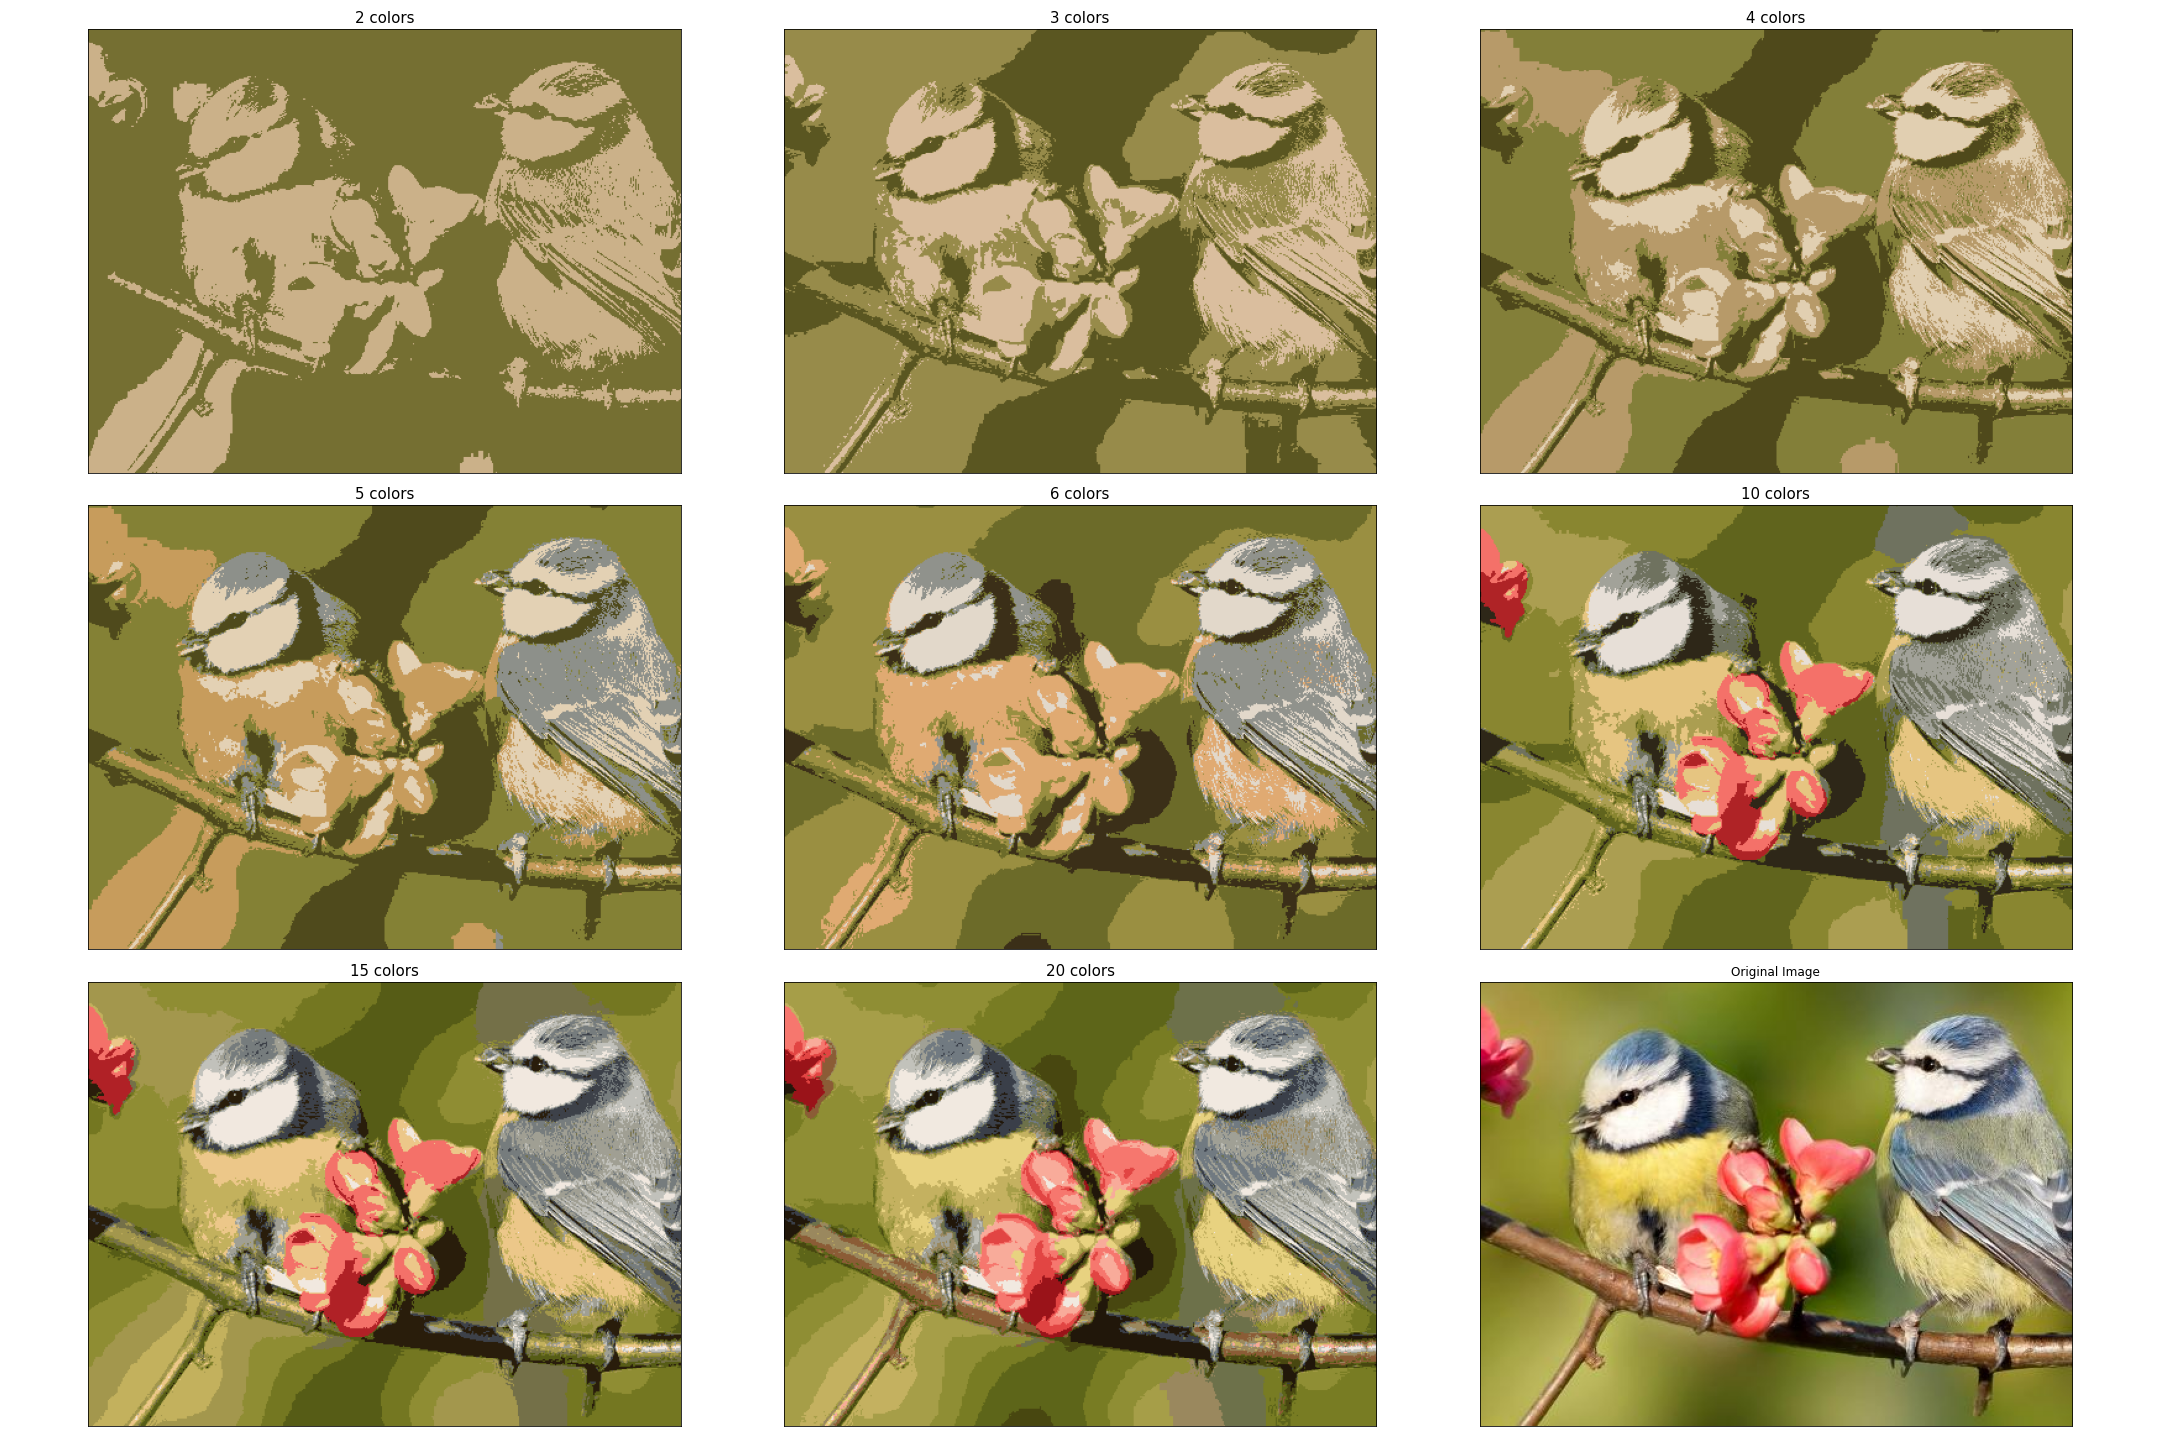
\includegraphics[width=0.8\linewidth]{images/q1/0.png}
    \caption{}
    \label{bird}
\end{figure}
\begin{figure}[h]
    \centering
    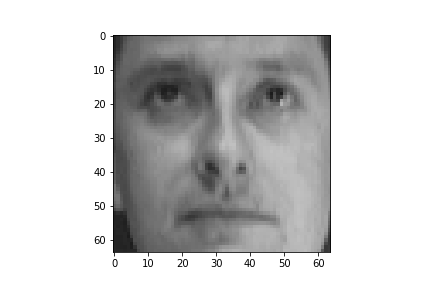
\includegraphics[width=0.8\linewidth]{images/q1/2.png}
    \caption{}
    \label{festival}
\end{figure}
\begin{figure}[h]
    \centering
    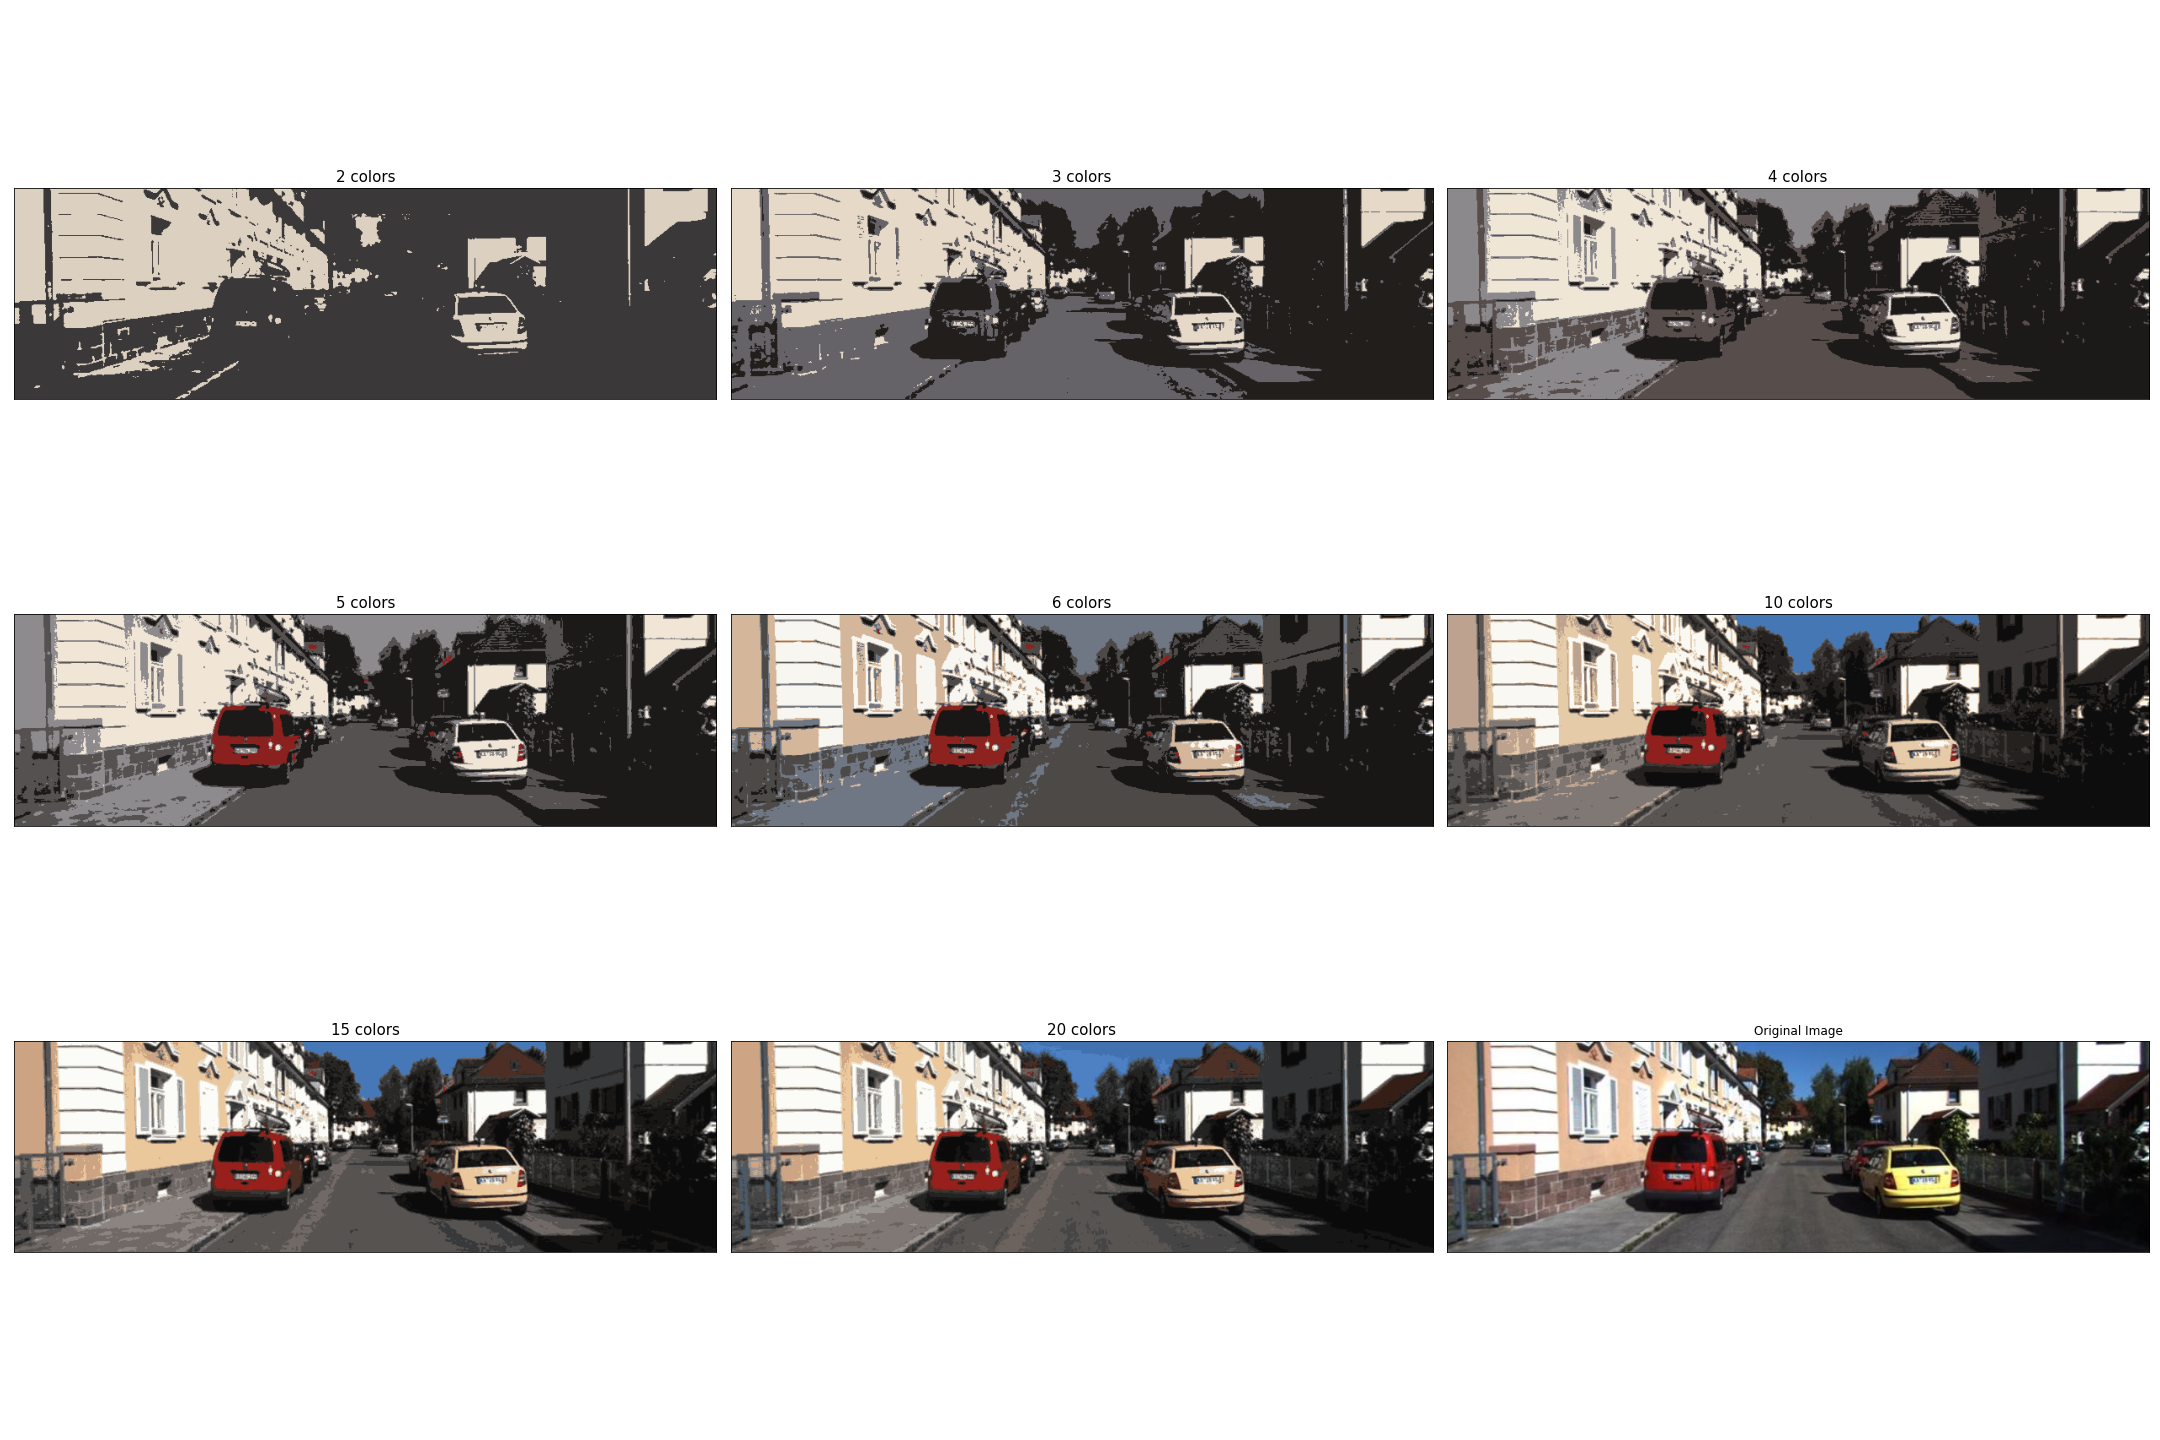
\includegraphics[width=\linewidth]{images/q1/1.png}
    \caption{}
    \label{car}
\end{figure}

\clearpage

\section*{سوال دو}

عملکرد الگوریتم \lr{DBSCAN} بر روی مجموعه دادگان در شکل \ref{dbscan} آورده شده است.
با وجود آن که پارامتر‌های مدل با سعی و خطا انتخاب شده است اما مدل عملکرد مناسبی را
به نمایش گذاشته است. به خصوص در مجموعه‌داده‌هایی مانند مارپیچ و حلقه که در آن‌ها پیوستگی بین
کلاس‌ها اهمیت بیشتری نسبت به جمع‌وجور بودن کلاس‌ها دارد. با همین دلیل عملکرد ضعیف الگوریتم
در مجموعه داده‌ی \lr{D31} قابل توجیه است.

\begin{figure}[h]
    \begin{subfigure}{0.45\linewidth}
        \centering
        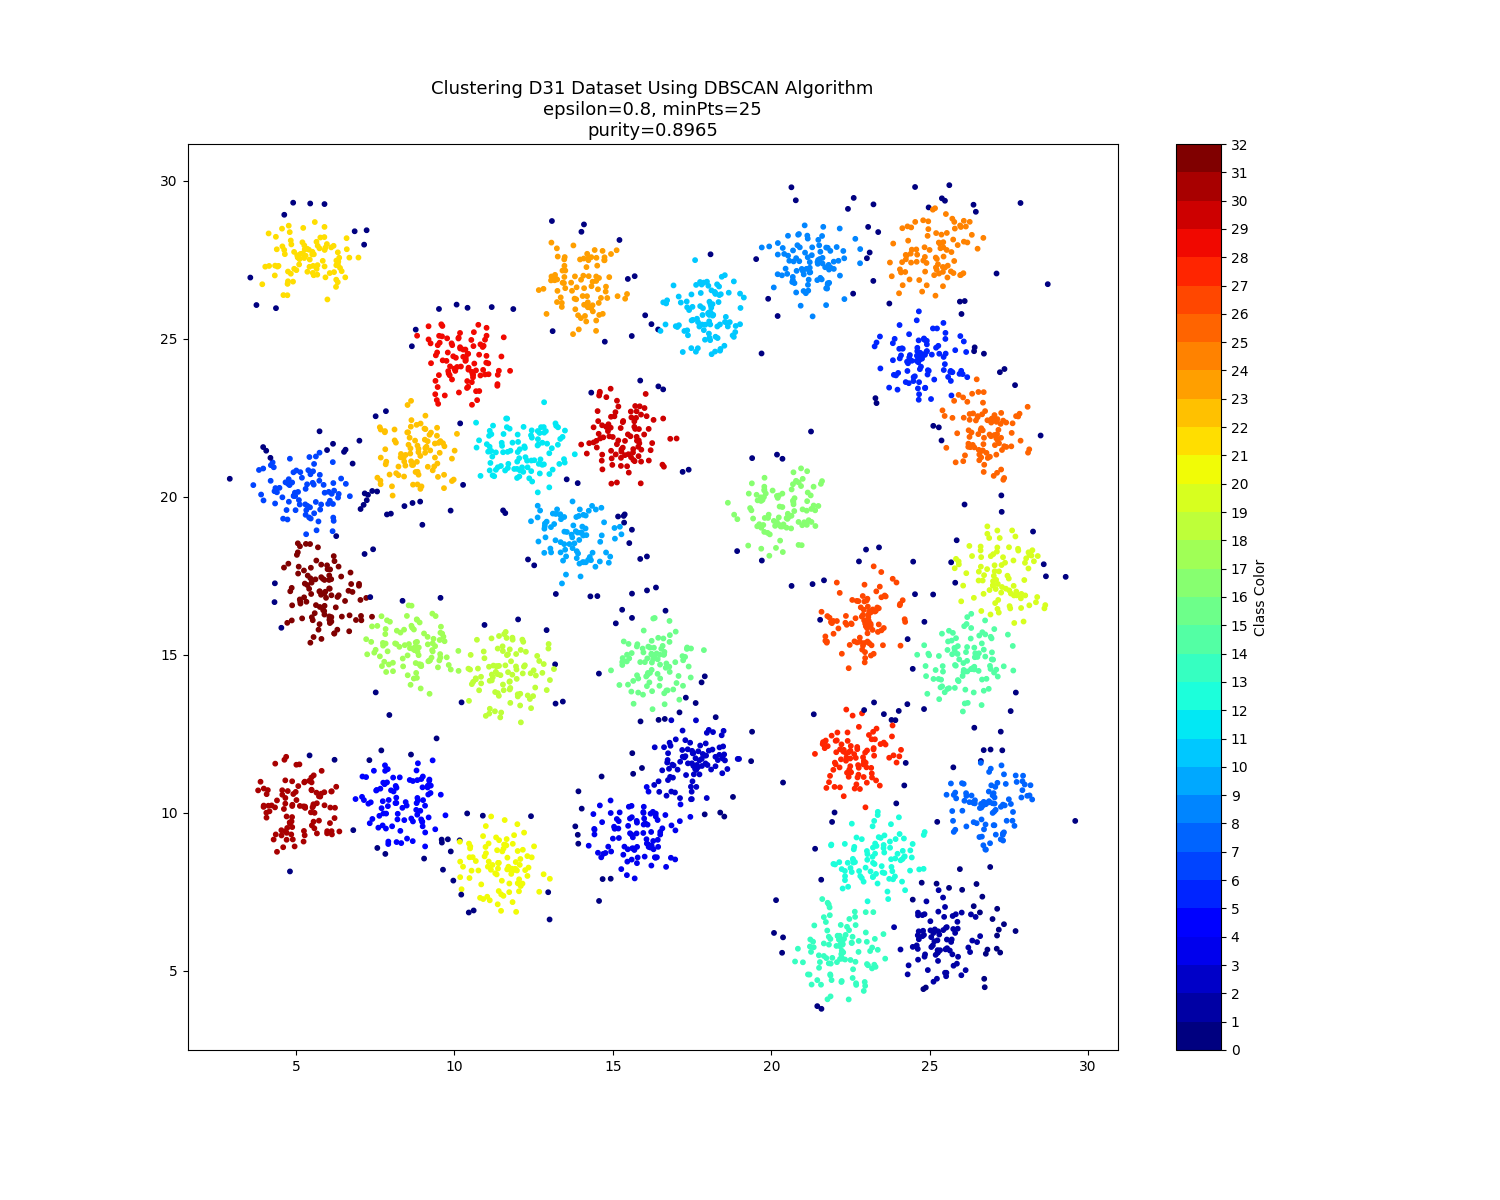
\includegraphics[width=0.8\linewidth]{images/q2/d31.png}
        \caption{}
        \label{d31}
    \end{subfigure}
    \hfill
    \begin{subfigure}{0.45\linewidth}
        \centering
        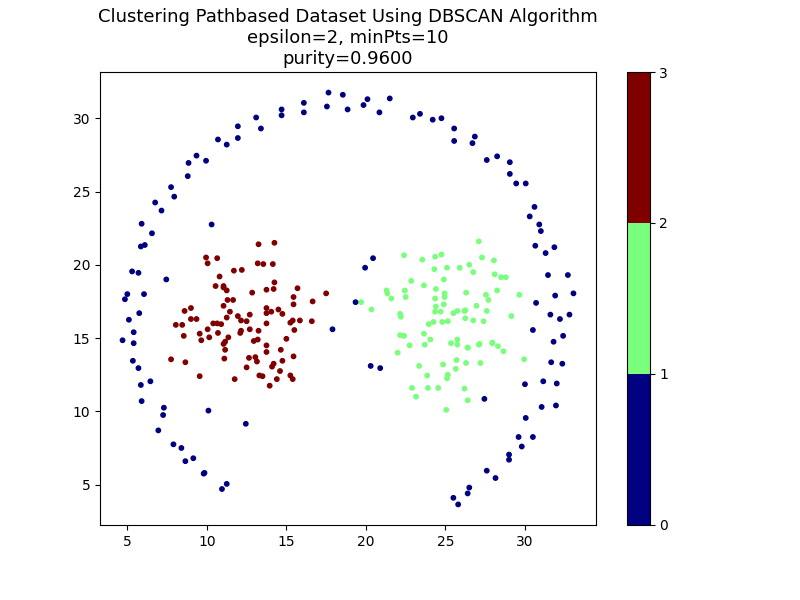
\includegraphics[width=0.8\linewidth]{images/q2/pathbased.png}
        \caption{}
        \label{pathbased}
    \end{subfigure}
    \newline
    \begin{subfigure}{0.45\linewidth}
        \centering
        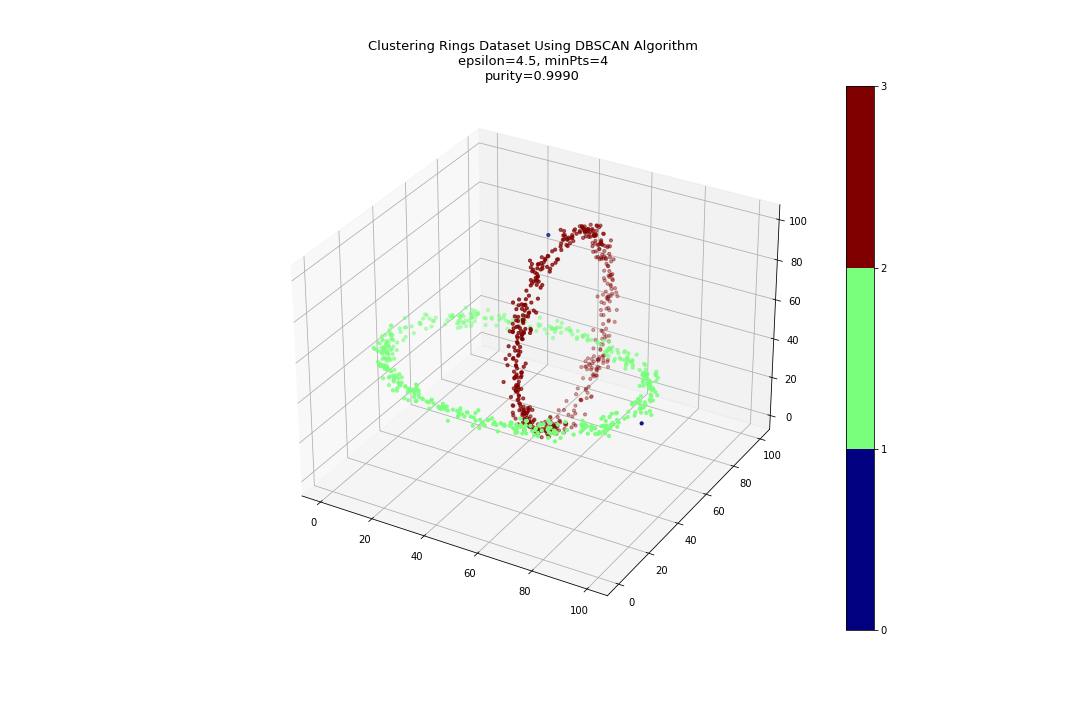
\includegraphics[width=\linewidth]{images/q2/rings.png}
        \caption{}
        \label{rings}
    \end{subfigure}
    \hfill
    \begin{subfigure}{0.45\linewidth}
        \centering
        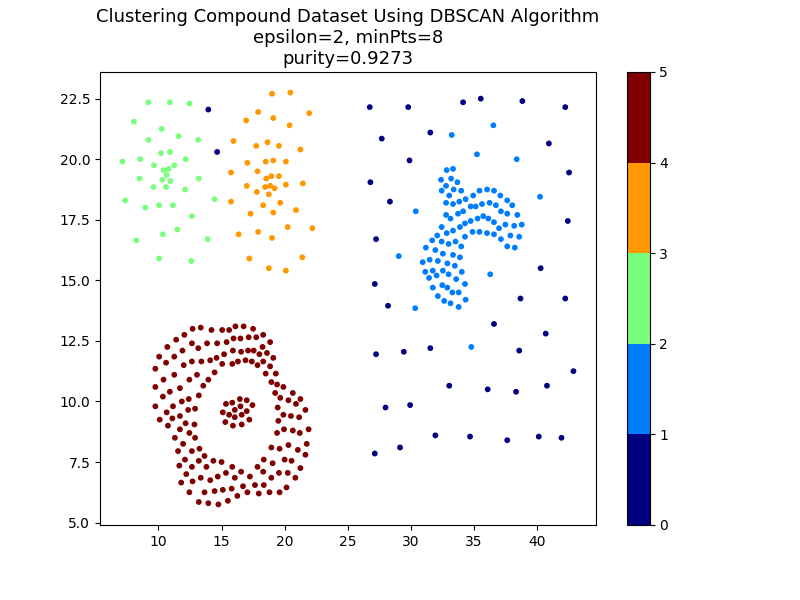
\includegraphics[width=\linewidth]{images/q2/compound.png}
        \caption{}
        \label{compound}
    \end{subfigure}
    \newline
    \hfill
    \begin{subfigure}{0.45\linewidth}
        \centering
        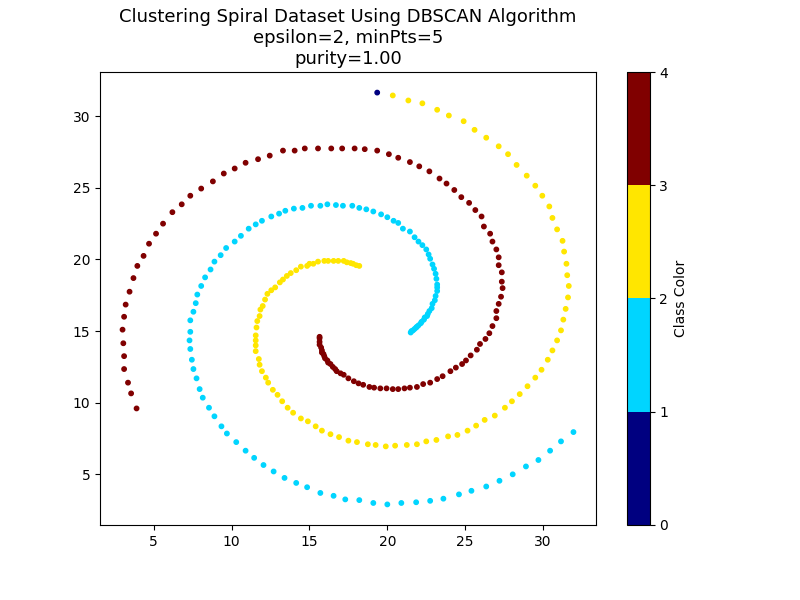
\includegraphics[width=\linewidth]{images/q2/spiral.png}
        \caption{}
        \label{spiral}
    \end{subfigure}
    \caption{}
    \label{dbscan}
\end{figure}

\clearpage

\section*{سوال سه}

\subsection*{قسمت الف}

در این نوع نمونه‌گیری ابتدا داده‌ها به دسته‌های همگون تقسیم می‌شوند. پس از تعیین سایز نمونه،
می‌توان به دو روش از این دسته‌های همگون داده انتخاب کرد.

\begin{itemize}
    \item \lr{Disproportionate Sampling}: در این روش از هر دسته به تعداد مساوی داده انتخاب می‌شود،
    بدون توجه به این که ممکن است تعداد داده موجود در هر دسته متفاوت باشد.
    \item \lr{Proportionate Sampling}: در این روش برخلاف روش قبلی، از هر دسته به نسبت داده‌های موجود در دسته
    داده انتخاب می‌شود. یعنی اگر تعداد داده موجود در یک دسته بیشتر باشد، سهم آن دسته در نمونه بیشتر خواهد بود.
\end{itemize}

مهم‌ترین حسن این نمونه‌گیری انتخاب بدون تعصب(\lr{bias}) از داده‌هاست.

\subsection*{قسمت ب}

نمودار \lr{elbow} با استفاده از الگوریتم خوشه‌بندی \lr{kmeans} در شکل \ref{elbow} مشاهده می‌شود.
همان‌طور که مشاهده می‌شود انتخاب عدد ۴۰ به عنوان تعداد خوشه‌های داده‌ها، قابل توجیه است.

\begin{figure}[h]
    \centering
    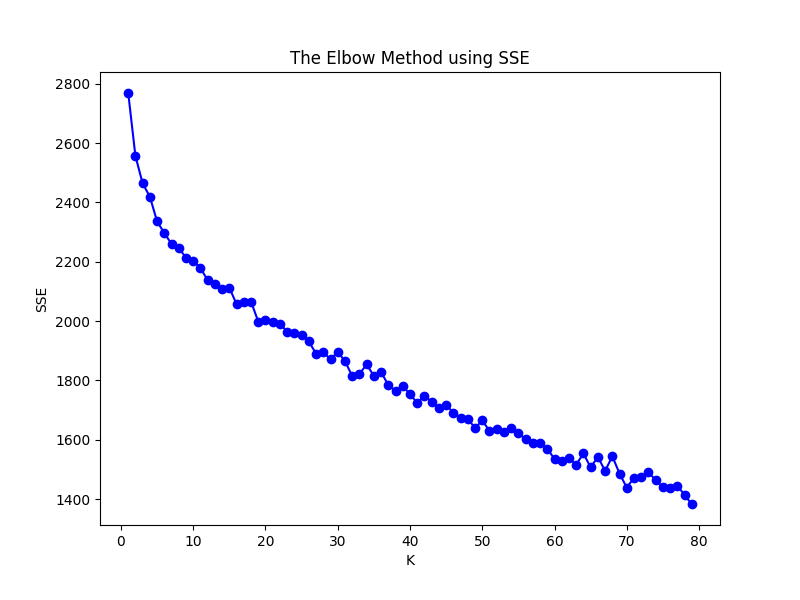
\includegraphics[width=0.8\linewidth]{images/q3/b/elbow.png}
    \caption{نمودار \lr{elbow} سوال ۳ قسمت ب}
    \label{elbow}
\end{figure}

\subsection*{قسمت ج}

در ادامه تصاویر متناظر هر یک خوشه‌‌ها آورده می‌شود. با توجه به زیاد بودن تعداد خوشه‌ها و تعداد تصاویر،
برای جلوگیری از افزایش حجم بی‌رویه گزارش تنها عکس‌های مربوط به ۱۰ خوشه آورده می‌شود.
در برخی از موارد تعداد داده‌های موجود در یک خوشه
کمتر از ۱۰ بود، برای این خوشه‌ها امکان آوردن ۱۰ نمونه تصویر از خوشه امکان‌پذیر نبود.
در باقی موارد تعداد ۱۰ تصویر به تصادف انتخاب شده و نمایش داده شده است.
همان‌طور که مشاهده می‌شود تصاویر موجود در خوشه‌ها به یکدیگر شبیه است اما مطابق انتظار
این الگوریتم نتوانسته است خوشه‌ها را به درستی تفکیک کند. چرا که برخی از تصاویر یک شخص را
یک خوشه و برخی دیگر را در یک خوشه دیگر. تفکیک داده‌ها به قسمت داده آموزشی، تست و ارزیابی
به نسبت 1، 1 و 8 بوده است.

\begin{figure}[h]
    \begin{subfigure}{0.3\linewidth}
        \centering
        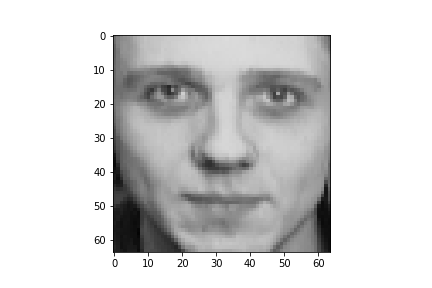
\includegraphics[width=\linewidth]{images/q3/c/0/0.png}
    \end{subfigure}
    \hfill
    \begin{subfigure}{0.3\linewidth}
        \centering
        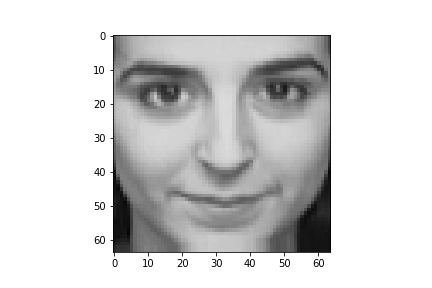
\includegraphics[width=\linewidth]{images/q3/c/0/1.png}
    \end{subfigure}
    \hfill
    \begin{subfigure}{0.3\linewidth}
        \centering
        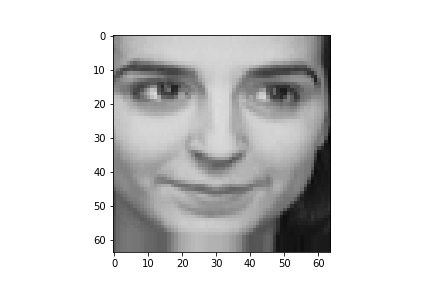
\includegraphics[width=\linewidth]{images/q3/c/0/2.png}
    \end{subfigure}
    \newline
    \begin{subfigure}{0.3\linewidth}
        \centering
        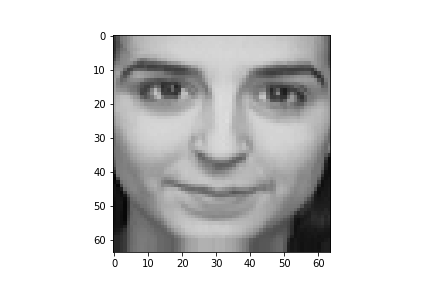
\includegraphics[width=\linewidth]{images/q3/c/0/3.png}
    \end{subfigure}
    \hfill
    \begin{subfigure}{0.3\linewidth}
        \centering
        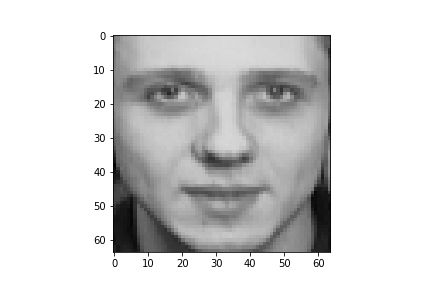
\includegraphics[width=\linewidth]{images/q3/c/0/4.png}
    \end{subfigure}
    \hfill
    \begin{subfigure}{0.3\linewidth}
        \centering
        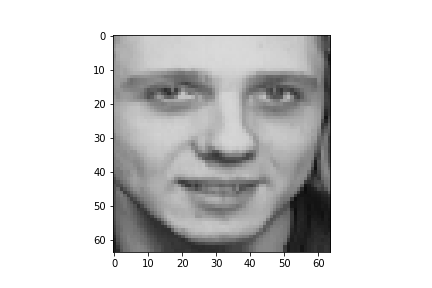
\includegraphics[width=\linewidth]{images/q3/c/0/5.png}
    \end{subfigure}
    \caption{خوشه اول}
\end{figure}

\begin{figure}[h]
    \begin{subfigure}{0.3\linewidth}
        \centering
        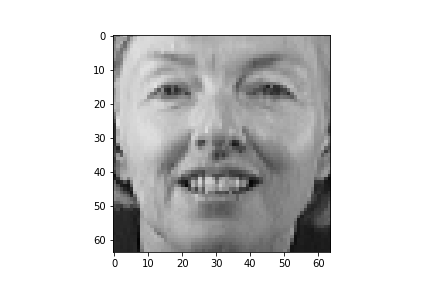
\includegraphics[width=\linewidth]{images/q3/c/1/0.png}
    \end{subfigure}
    \hfill
    \begin{subfigure}{0.3\linewidth}
        \centering
        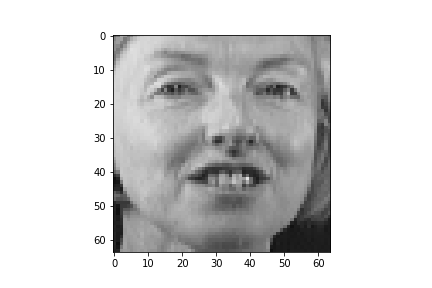
\includegraphics[width=\linewidth]{images/q3/c/1/1.png}
    \end{subfigure}
    \hfill
    \begin{subfigure}{0.3\linewidth}
        \centering
        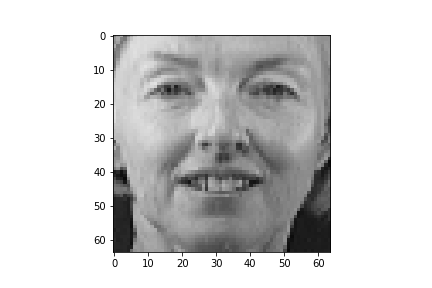
\includegraphics[width=\linewidth]{images/q3/c/1/2.png}
    \end{subfigure}
    \caption{خوشه دوم}
\end{figure}

\begin{figure}[h]
    \begin{subfigure}{0.3\linewidth}
        \centering
        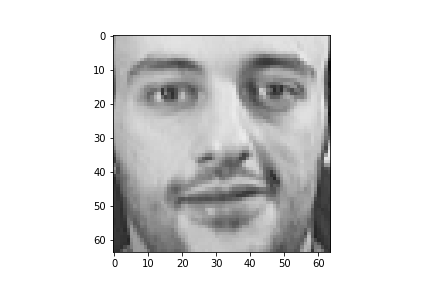
\includegraphics[width=\linewidth]{images/q3/c/2/0.png}
    \end{subfigure}
    \hfill
    \begin{subfigure}{0.3\linewidth}
        \centering
        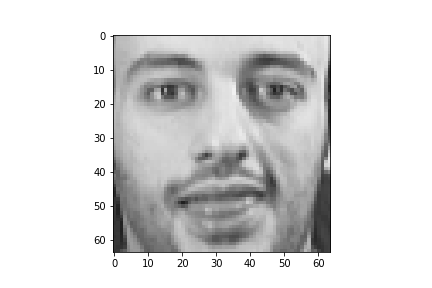
\includegraphics[width=\linewidth]{images/q3/c/2/1.png}
    \end{subfigure}
    \hfill
    \caption{خوشه سوم}
\end{figure}

\clearpage

\begin{figure}[h]
    \begin{subfigure}{0.3\linewidth}
        \centering
        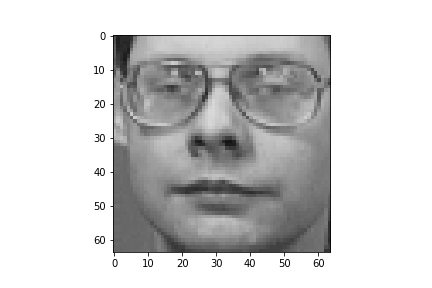
\includegraphics[width=\linewidth]{images/q3/c/3/0.png}
    \end{subfigure}
    \hfill
    \begin{subfigure}{0.3\linewidth}
        \centering
        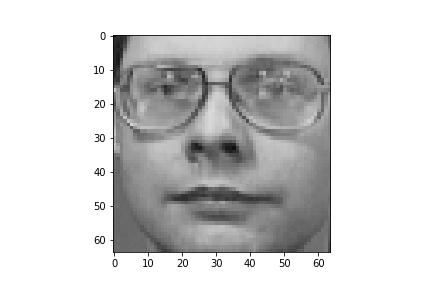
\includegraphics[width=\linewidth]{images/q3/c/3/1.png}
    \end{subfigure}
    \hfill
    \begin{subfigure}{0.3\linewidth}
        \centering
        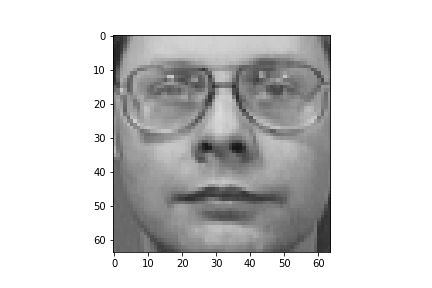
\includegraphics[width=\linewidth]{images/q3/c/3/2.png}
    \end{subfigure}
    \caption{خوشه چهارم}
\end{figure}

\begin{figure}[h]
    \begin{subfigure}{0.3\linewidth}
        \centering
        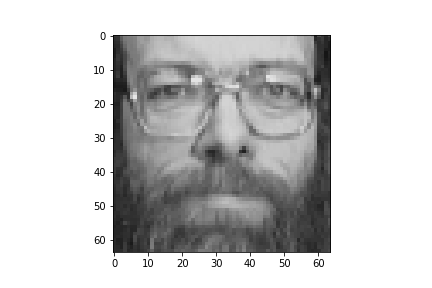
\includegraphics[width=\linewidth]{images/q3/c/4/0.png}
    \end{subfigure}
    \hfill
    \begin{subfigure}{0.3\linewidth}
        \centering
        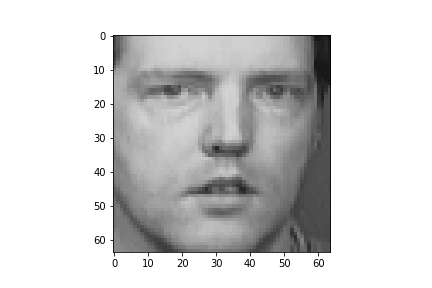
\includegraphics[width=\linewidth]{images/q3/c/4/1.png}
    \end{subfigure}
    \hfill
    \begin{subfigure}{0.3\linewidth}
        \centering
        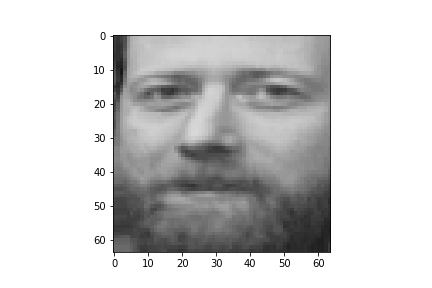
\includegraphics[width=\linewidth]{images/q3/c/4/2.png}
    \end{subfigure}
    \newline
    \begin{subfigure}{0.3\linewidth}
        \centering
        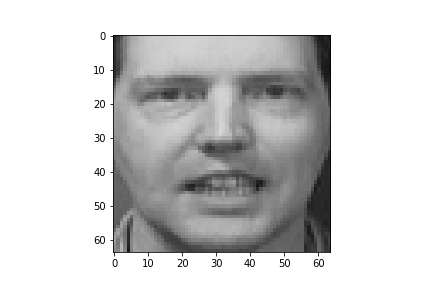
\includegraphics[width=\linewidth]{images/q3/c/4/3.png}
    \end{subfigure}
    \hfill
    \begin{subfigure}{0.3\linewidth}
        \centering
        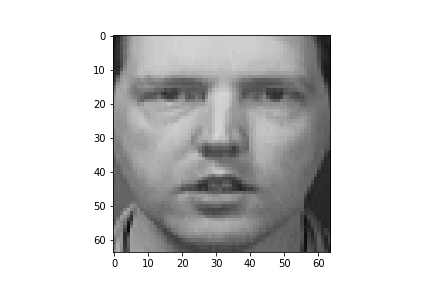
\includegraphics[width=\linewidth]{images/q3/c/4/4.png}
    \end{subfigure}
    \hfill
    \begin{subfigure}{0.3\linewidth}
        \centering
        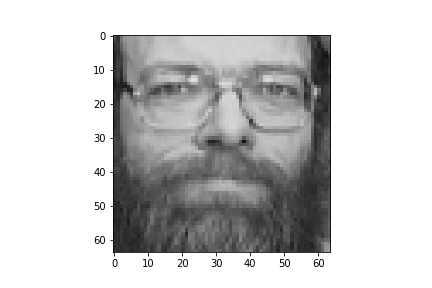
\includegraphics[width=\linewidth]{images/q3/c/4/5.png}
    \end{subfigure}
    \newline
    \begin{subfigure}{0.3\linewidth}
        \centering
        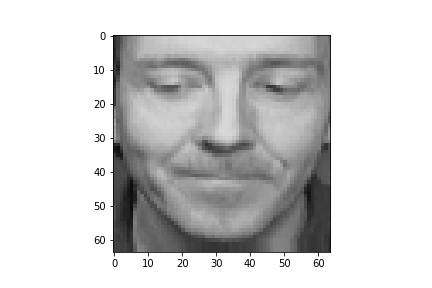
\includegraphics[width=\linewidth]{images/q3/c/4/6.png}
    \end{subfigure}
    \hfill
    \begin{subfigure}{0.3\linewidth}
        \centering
        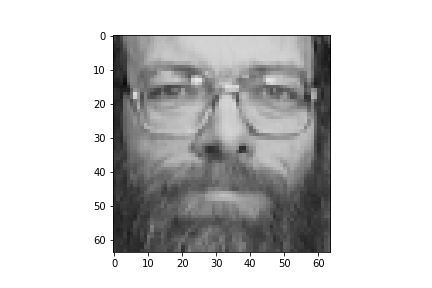
\includegraphics[width=\linewidth]{images/q3/c/4/7.png}
    \end{subfigure}
    \hfill
    \begin{subfigure}{0.3\linewidth}
        \centering
        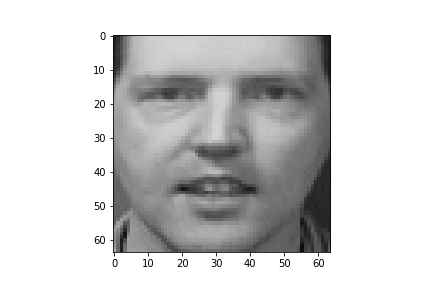
\includegraphics[width=\linewidth]{images/q3/c/4/8.png}
    \end{subfigure}
    \newline
    \hfill
    \begin{subfigure}{0.3\linewidth}
        \centering
        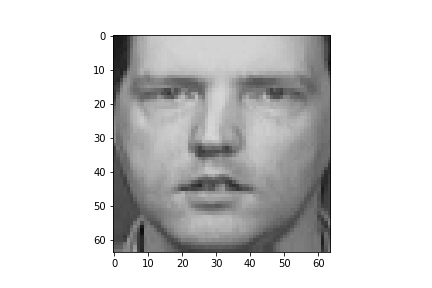
\includegraphics[width=\linewidth]{images/q3/c/4/9.png}
    \end{subfigure}
    \caption{خوشه پنجم}
\end{figure}

\clearpage

\begin{figure}[h]
    \begin{subfigure}{0.3\linewidth}
        \centering
        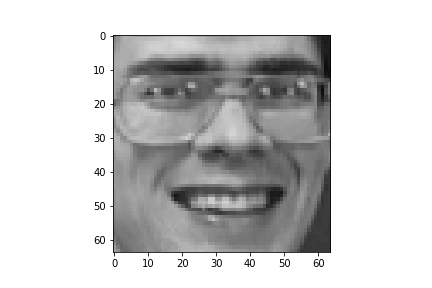
\includegraphics[width=\linewidth]{images/q3/c/5/0.png}
    \end{subfigure}
    \hfill
    \begin{subfigure}{0.3\linewidth}
        \centering
        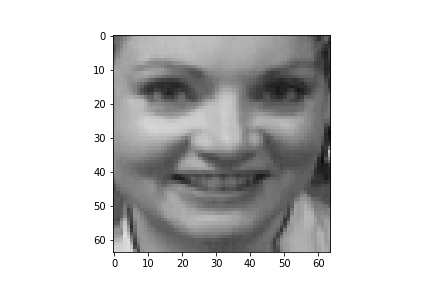
\includegraphics[width=\linewidth]{images/q3/c/5/1.png}
    \end{subfigure}
    \hfill
    \begin{subfigure}{0.3\linewidth}
        \centering
        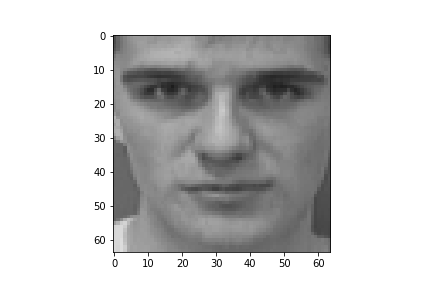
\includegraphics[width=\linewidth]{images/q3/c/5/2.png}
    \end{subfigure}
    \newline
    \begin{subfigure}{0.3\linewidth}
        \centering
        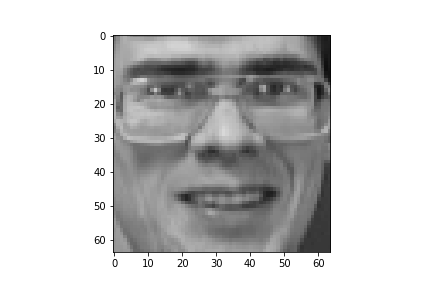
\includegraphics[width=\linewidth]{images/q3/c/5/3.png}
    \end{subfigure}
    \hfill
    \begin{subfigure}{0.3\linewidth}
        \centering
        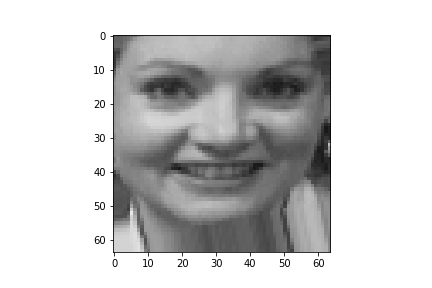
\includegraphics[width=\linewidth]{images/q3/c/5/4.png}
    \end{subfigure}
    \hfill
    \begin{subfigure}{0.3\linewidth}
        \centering
        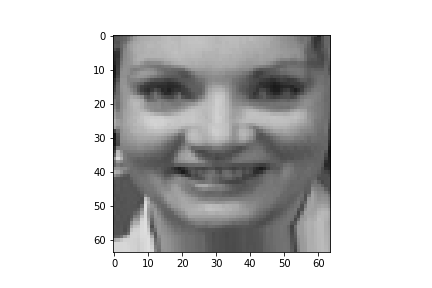
\includegraphics[width=\linewidth]{images/q3/c/5/5.png}
    \end{subfigure}
    \newline
    \begin{subfigure}{0.3\linewidth}
        \centering
        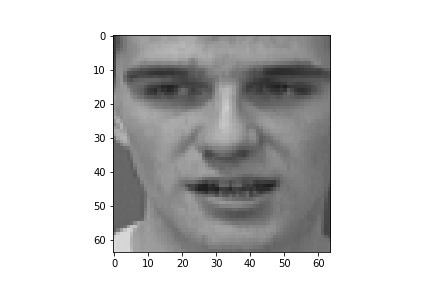
\includegraphics[width=\linewidth]{images/q3/c/5/6.png}
    \end{subfigure}
    \hfill
    \begin{subfigure}{0.3\linewidth}
        \centering
        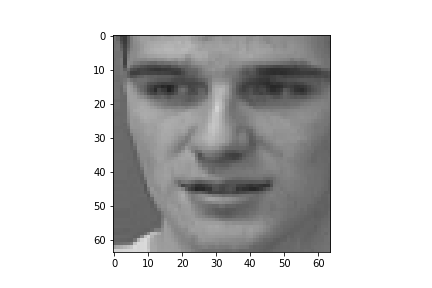
\includegraphics[width=\linewidth]{images/q3/c/5/7.png}
    \end{subfigure}
    \hfill
    \begin{subfigure}{0.3\linewidth}
        \centering
        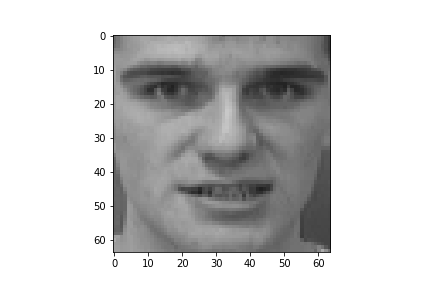
\includegraphics[width=\linewidth]{images/q3/c/5/8.png}
    \end{subfigure}
    \newline
    \hfill
    \begin{subfigure}{0.3\linewidth}
        \centering
        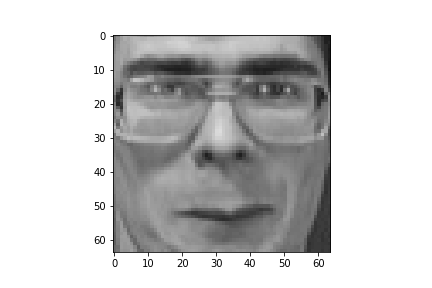
\includegraphics[width=\linewidth]{images/q3/c/5/9.png}
    \end{subfigure}
    \caption{خوشه ششم}
\end{figure}

\clearpage

\begin{figure}[h]
    \begin{subfigure}{0.3\linewidth}
        \centering
        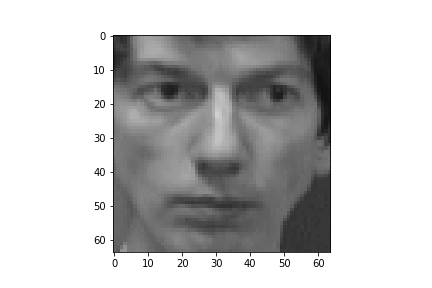
\includegraphics[width=\linewidth]{images/q3/c/6/0.png}
    \end{subfigure}
    \hfill
    \begin{subfigure}{0.3\linewidth}
        \centering
        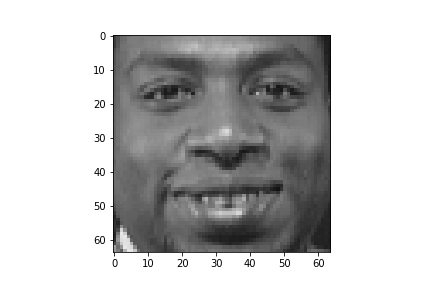
\includegraphics[width=\linewidth]{images/q3/c/6/1.png}
    \end{subfigure}
    \hfill
    \begin{subfigure}{0.3\linewidth}
        \centering
        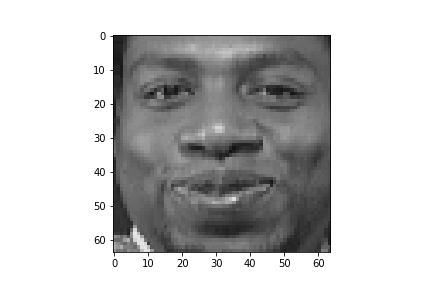
\includegraphics[width=\linewidth]{images/q3/c/6/2.png}
    \end{subfigure}
    \newline
    \begin{subfigure}{0.3\linewidth}
        \centering
        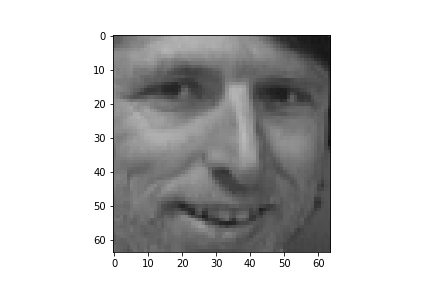
\includegraphics[width=\linewidth]{images/q3/c/6/3.png}
    \end{subfigure}
    \hfill
    \begin{subfigure}{0.3\linewidth}
        \centering
        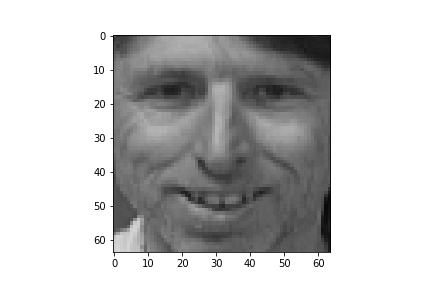
\includegraphics[width=\linewidth]{images/q3/c/6/4.png}
    \end{subfigure}
    \hfill
    \begin{subfigure}{0.3\linewidth}
        \centering
        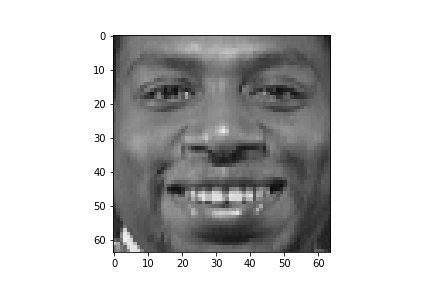
\includegraphics[width=\linewidth]{images/q3/c/6/5.png}
    \end{subfigure}
    \newline
    \begin{subfigure}{0.3\linewidth}
        \centering
        \includegraphics[width=\linewidth]{images/q3/c/6/6.png}
    \end{subfigure}
    \hfill
    \begin{subfigure}{0.3\linewidth}
        \centering
        \includegraphics[width=\linewidth]{images/q3/c/6/7.png}
    \end{subfigure}
    \hfill
    \begin{subfigure}{0.3\linewidth}
        \centering
        \includegraphics[width=\linewidth]{images/q3/c/6/8.png}
    \end{subfigure}
    \newline
    \hfill
    \begin{subfigure}{0.3\linewidth}
        \centering
        \includegraphics[width=\linewidth]{images/q3/c/6/9.png}
    \end{subfigure}
    \caption{خوشه هفتم}
\end{figure}

\clearpage

\begin{figure}[h]
    \begin{subfigure}{0.3\linewidth}
        \centering
        \includegraphics[width=\linewidth]{images/q3/c/7/0.png}
    \end{subfigure}
    \hfill
    \begin{subfigure}{0.3\linewidth}
        \centering
        \includegraphics[width=\linewidth]{images/q3/c/7/1.png}
    \end{subfigure}
    \hfill
    \begin{subfigure}{0.3\linewidth}
        \centering
        \includegraphics[width=\linewidth]{images/q3/c/7/2.png}
    \end{subfigure}
    \newline
    \begin{subfigure}{0.3\linewidth}
        \centering
        \includegraphics[width=\linewidth]{images/q3/c/7/3.png}
    \end{subfigure}
    \hfill
    \begin{subfigure}{0.3\linewidth}
        \centering
        \includegraphics[width=\linewidth]{images/q3/c/7/4.png}
    \end{subfigure}
    \hfill
    \begin{subfigure}{0.3\linewidth}
        \centering
        \includegraphics[width=\linewidth]{images/q3/c/7/5.png}
    \end{subfigure}
    \newline
    \begin{subfigure}{0.3\linewidth}
        \centering
        \includegraphics[width=\linewidth]{images/q3/c/7/6.png}
    \end{subfigure}
    \hfill
    \begin{subfigure}{0.3\linewidth}
        \centering
        \includegraphics[width=\linewidth]{images/q3/c/7/7.png}
    \end{subfigure}
    \hfill
    \begin{subfigure}{0.3\linewidth}
        \centering
        \includegraphics[width=\linewidth]{images/q3/c/7/8.png}
    \end{subfigure}
    \caption{خوشه هشتم}
\end{figure}

\clearpage

\begin{figure}[h]
    \begin{subfigure}{0.3\linewidth}
        \centering
        \includegraphics[width=\linewidth]{images/q3/c/8/0.png}
    \end{subfigure}
    \hfill
    \begin{subfigure}{0.3\linewidth}
        \centering
        \includegraphics[width=\linewidth]{images/q3/c/8/1.png}
    \end{subfigure}
    \hfill
    \begin{subfigure}{0.3\linewidth}
        \centering
        \includegraphics[width=\linewidth]{images/q3/c/8/2.png}
    \end{subfigure}
    \newline
    \begin{subfigure}{0.3\linewidth}
        \centering
        \includegraphics[width=\linewidth]{images/q3/c/8/3.png}
    \end{subfigure}
    \hfill
    \begin{subfigure}{0.3\linewidth}
        \centering
        \includegraphics[width=\linewidth]{images/q3/c/8/4.png}
    \end{subfigure}
    \hfill
    \begin{subfigure}{0.3\linewidth}
        \centering
        \includegraphics[width=\linewidth]{images/q3/c/8/5.png}
    \end{subfigure}
    \newline
    \begin{subfigure}{0.3\linewidth}
        \centering
        \includegraphics[width=\linewidth]{images/q3/c/8/6.png}
    \end{subfigure}
    \hfill
    \begin{subfigure}{0.3\linewidth}
        \centering
        \includegraphics[width=\linewidth]{images/q3/c/8/7.png}
    \end{subfigure}
    \hfill
    \begin{subfigure}{0.3\linewidth}
        \centering
        \includegraphics[width=\linewidth]{images/q3/c/8/8.png}
    \end{subfigure}
    \newline
    \hfill
    \begin{subfigure}{0.3\linewidth}
        \centering
        \includegraphics[width=\linewidth]{images/q3/c/8/9.png}
    \end{subfigure}
    \caption{خوشه نهم}
\end{figure}

\begin{figure}[h]
    \begin{subfigure}{0.3\linewidth}
        \centering
        \includegraphics[width=\linewidth]{images/q3/c/9/0.png}
    \end{subfigure}
    \hfill
    \begin{subfigure}{0.3\linewidth}
        \centering
        \includegraphics[width=\linewidth]{images/q3/c/9/1.png}
    \end{subfigure}
    \hfill
    \begin{subfigure}{0.3\linewidth}
        \centering
        \includegraphics[width=\linewidth]{images/q3/c/9/2.png}
    \end{subfigure}
    \newline
    \begin{subfigure}{0.3\linewidth}
        \centering
        \includegraphics[width=\linewidth]{images/q3/c/9/3.png}
    \end{subfigure}
    \hfill
    \begin{subfigure}{0.3\linewidth}
        \centering
        \includegraphics[width=\linewidth]{images/q3/c/9/4.png}
    \end{subfigure}
    \hfill
    \begin{subfigure}{0.3\linewidth}
        \centering
        \includegraphics[width=\linewidth]{images/q3/c/9/5.png}
    \end{subfigure}
    \caption{خوشه دهم}
\end{figure}

\clearpage

\section*{سوال چهارم}

\subsection*{قسمت الف}

نتیجه به شکل زیر حاصل می‌شود. (شکل‌های \ref{parta_policy} و \ref{parta_value})

\begin{figure}[h]
    \centering
    \includegraphics{images/q4/a/policy.png}
    \caption{}
    \label{parta_policy}
\end{figure}

\begin{figure}[h]
    \centering
    \includegraphics[width=0.8\linewidth]{images/q4/a/value.png}
    \caption{}
    \label{parta_value}
\end{figure}

\clearpage

\subsection*{قسمت ب}

نتایج این قسمت در شکل \ref{partb_policy} و \ref{partb_value} دیده می‌شود.
در این حالت با توجه به عدم وجود اصطکاک انتظار می‌رفت که ربات مدت بیشتری را در
محیط بگذراند و آرام‌تر به سمت هدف برود. اما همان‌طور که مشاهده می‌شود تغییری در
عملکرد ربات دیده نمی‌شود. البته عملکرد ربات همچنان قابل توجیه است. برای توجیه این عملکرد
مقادیر ارزشی که برای هر خانه از محیط در نظر گرفته شده است را با هم مقایسه می‌کنیم.
همان‌طور که مشاهده می‌شود تفاوت چندانی در مقادیر ارزش در نظر گرفته شده برای هر خانه
در این حالت با حالت قبلی دیده نمی‌شود. دلیل این امر کم‌بودن میزان اصطکاک در قسمت الف سوال است.
به دلیل همین یکسانی جدول ارزش‌دهی حالت‌ها، در نتیجه سیاست‌گذاری انجام شده نیز یکسان شده
است.

البته در هنگام چاپ مقادیر ارزش برای هر خانه، تنها مقدار صحیح آن در نظر گرفته شده است.
نکته دیگری که در هنگام پیاده‌سازی لحاظ شده است، باقی‌ماندن ربات در خانه نهایی است. بدین معنی که
اگر ربات وارد خانه نهایی شود، هر حرکتی انجام دهد نمی‌تواند از آن خانه خارج شود.

\begin{figure}[h]
    \centering
    \includegraphics{images/q4/b/policy.png}
    \caption{}
    \label{partb_policy}
\end{figure}

\begin{figure}[h]
    \centering
    \includegraphics[width=0.8\linewidth]{images/q4/b/value.png}
    \caption{}
    \label{partb_value}
\end{figure}

\clearpage

\subsection*{قسمت ج}

نتایج این قسمت در شکل‌های \ref{partc_policy} و \ref{partc_value} مشاهده می‌شود. در این قسمت نیز تفاوتی بین
این نتایج با نتایج قسمت‌های قبلی دیده می‌شود. در این حالت با توجه به زیاد بودن مقدار اصطکاک ازرش‌گذاری خانه‌ها
به وضوح افت کرده است. اما سیاست در نظر گرفته شده یکسان است. دلیل این اتفاق به ماهیت عملکرد ربات بازمی‌گردد.
هدف ربات رسیدن به خانه هدف است. خانه هدف نیز بیشترین عاید را برای او دارد. بنابراین چرا باید راه مستقیم را
رها کرده و بی‌دلیل در محیط بچرخد؟!

\begin{figure}[h]
    \centering
    \includegraphics[scale=0.9]{images/q4/c/policy.png}
    \caption{}
    \label{partc_policy}
\end{figure}

\begin{figure}[h]
    \centering
    \includegraphics[width=0.8\linewidth]{images/q4/c/value.png}
    \caption{}
    \label{partc_value}
\end{figure}

\clearpage

\subsection*{قسمت د}

در ادامه نقش مقادیر مختلف \lr{discount factor} در محیط حالت پایه بررسی می‌شود.
(شکل \ref{base_env}) همان‌طور که مشاهده می‌شود، هر چه مقدار \lr{discount} کم‌تر می‌شود،
ربات از پاداش نهایی که در انتظارش است غافل شده و به پاداش‌های لحظه‌ای بیشتر اهمیت می‌دهد.
همین دلیل باعث می‌شود که ربات ترجیح دهد در حالت فعلی خود باقی بماند تا مجبور نشود هزینه
حرکت را بپردازد.

\begin{figure}[h]
    \begin{subfigure}{0.45\linewidth}
        \centering
        \includegraphics[width=\linewidth]{images/q4/d/base/discount_09.png}
        \caption{\lr{$\text{discount} = 0.9$}}
    \end{subfigure}
    \hfill
    \begin{subfigure}{0.45\linewidth}
        \centering
        \includegraphics[width=\linewidth]{images/q4/d/base/discount_75.png}
        \caption{\lr{$\text{discount} = 0.75$}}
    \end{subfigure}
    \newline
    \begin{subfigure}{0.45\linewidth}
        \centering
        \includegraphics[width=\linewidth]{images/q4/d/base/discount_05.png}
        \caption{\lr{$\text{discount} = 0.5$}}
    \end{subfigure}
    \hfill
    \begin{subfigure}{0.45\linewidth}
        \centering
        \includegraphics[width=\linewidth]{images/q4/d/base/discount_01.png}
        \caption{\lr{$\text{discount} = 0.1$}}
    \end{subfigure}
    \caption{تاثیر مقادیر مختلف \lr{discount} در آینده‌نگری ربات در محیط پایه}
    \label{base_env}
\end{figure}

\clearpage

نتایج در شکل \ref{nocost_env} مشاهده می‌شود. از آن جا که در این محیط حرکت‌کردن هزینه‌ای ندارد،
بنابراین ربات با حرکت‌کردن متحمل شدن هیچ ضرری نمی‌شود. در نتیجه می‌تواند حالت پایانی
را نیز پیدا کند. به همین دلیل حتی اگر مقدار \lr{dicsount} را بسیار کم نیز در نظر گرفته و ربات را به
پاداش‌های لحظه‌ای خرسند کنیم، ربات می‌تواند سیاست بهینه را یاد بگیرد. البته با کم کردن مقدار \lr{discount}
ارزش در نظر گرفته برای هر خانه بسیار کم و در حد $10^{-12}$ می‌شود. اما سیاست بهینه با مقایسه همین مقادیر
اندک، قابل حصول است.

\begin{figure}[h]
    \begin{subfigure}{0.45\linewidth}
        \centering
        \includegraphics[width=\linewidth]{images/q4/d/nocost/discount_09.png}
        \caption{\lr{$\text{discount} = 0.9$}}
    \end{subfigure}
    \hfill
    \begin{subfigure}{0.45\linewidth}
        \centering
        \includegraphics[width=\linewidth]{images/q4/d/nocost/discount_75.png}
        \caption{\lr{$\text{discount} = 0.75$}}
    \end{subfigure}
    \newline
    \begin{subfigure}{0.45\linewidth}
        \centering
        \includegraphics[width=\linewidth]{images/q4/d/nocost/discount_05.png}
        \caption{\lr{$\text{discount} = 0.5$}}
    \end{subfigure}
    \hfill
    \begin{subfigure}{0.45\linewidth}
        \centering
        \includegraphics[width=\linewidth]{images/q4/d/nocost/discount_01.png}
        \caption{\lr{$\text{discount} = 0.1$}}
    \end{subfigure}
    \caption{تاثیر مقادیر مختلف \lr{discount} در آینده‌نگری ربات در محیط بدون اصطکاک}
    \label{nocost_env}
\end{figure}

\clearpage

\subsection*{قسمت ه}

در اجراهای الگوریتم \lr{value iteration} در حالت‌های پایه، بدون اصطکاک و با اصطکاک زیاد به جواب
بهینه می‌رسیم. این جواب بهینه همان جوابی است که در قسمت‌های قبلی و با استفاده از الگوریتم
\lr{policy iteration} حاصل شده بودند. نتایج به دست آمده در این حالت نیز منطقی بوده و ربات تلاش می‌کند
با حرکت بر یک خط مستقیم و در نزدیک‌ترین زمان ممکن به هدف خود برسد. نتایج این قسمت در شکل‌های
\ref{value_iter_base}، \ref{value_iter_nocost} و \ref{value_iter_highcost} دیده می‌شود.

\begin{figure}[h]
    \begin{subfigure}{\linewidth}
        \centering
        \includegraphics{images/q4/e/base/policy.png}
        \caption{سیاست}
    \end{subfigure}
    \newline
    \begin{subfigure}{\linewidth}
        \centering
        \includegraphics[width=\linewidth]{images/q4/e/base/value.png}
        \caption{ارزش‌گذاری}
    \end{subfigure}
    \caption{سیاست و ارزش‌گذاری بهینه با استفاده از الگوریتم \lr{value iteration} در محیط پایه}
    \label{value_iter_base}
\end{figure}

\clearpage

\begin{figure}
    \begin{subfigure}{\linewidth}
        \centering
        \includegraphics{images/q4/e/nocost/policy.png}
        \caption{سیاست}
    \end{subfigure}
    \newline
    \begin{subfigure}{\linewidth}
        \centering
        \includegraphics[width=\linewidth]{images/q4/e/nocost/value.png}
        \caption{ارزش‌گذاری}
    \end{subfigure}
    \caption{سیاست و ارزش‌گذاری بهینه با استفاده از الگوریتم \lr{value iteration} در محیط بدون اصطکاک}
    \label{value_iter_nocost}
\end{figure}

\clearpage

\begin{figure}
    \begin{subfigure}{\linewidth}
        \centering
        \includegraphics{images/q4/e/highcost/policy.png}
        \caption{سیاست}
    \end{subfigure}
    \newline
    \begin{subfigure}{\linewidth}
        \centering
        \includegraphics[width=\linewidth]{images/q4/e/highcost/value.png}
        \caption{ارزش‌گذاری}
    \end{subfigure}
    \caption{سیاست و ارزش‌گذاری بهینه با استفاده از الگوریتم \lr{value iteration} در محیط با اصطکاک بالا}
    \label{value_iter_highcost}
\end{figure}

\end{document}